\chapter{ガイダンス}

\section{はじめに}
パソコン(Personal Computer) は、文字通りパーソナル・個人的に一人で一台を独占して利用することを前提に作られている。
例えば、あなたが友達のパソコンを使う機会があったとする。
あなたが昨日、自分のパソコンで作った文章を友達のパソコン上でちょっと編集して新しい文章を作りたいと思ったとしても、
あなたのパソコンは遠く離れたあなたの家にあり、わざわざ家に帰って、CD や USB メモリに保存し、もう一度持ってこなくてはならない。

これに対してメディアセンターには、一つの部屋に何台ものパソコンが並んでいる。例えば、この演習室には約60台のパソコンが並んでいる。
仮に、これらのパソコンにNo. 1 から順に番号をつけるとする。ある日、あなたが No. 7 のパソコンを使って、自分宛の電子メールを読んだり、ワープロでレポートを書いたりしたとすると、このときのデータはNo. 7 のパソコン上に保存され(るように見え)る。次の日にあなたが演習室に来てみると、No. 7 のパソコンはすでに他の人に使われていた。
このような時でも、No. 7 のパソコン上に保存した(ように見えた)あなたの電子メールは他人に読まれることはないし、レポートの続きを書くためにNo. 7 のパソコンが空くまで待つ必要もない。演習室の別のパソコン、例えば、No. 51 のパソコンを使って、続きの作業をすることができる。
これが、メディアセンターのパソコンの最大の特徴である。あたかも、自分一人だけのパソコンのように内容の秘密を保ちながら、どのパソコンを使っても同様の作業環境が提供されている。この特徴は、この演習室内のパソコンにとどまらず、大学内のあちこちに設置されているメディアセンターすべてのパソコンについて実現されている。このようなパソコンをPC端末と言う。

PC端末(教育用コンピュータシステム)の基本的な使い方は、京都大学情報環境機構のホームページに「学生のための情報環境活用マニュアル」(pdf ファイル)があるので、これを参照してもよい。

\url{http://www.iimc.kyoto-u.ac.jp/ja/services/ecs/support/tebiki.html}

このような環境を実現するために、メディアセンターではサーバと呼ばれる大きな一つのパソコンに各PC端末がつながっているシステムを形成している。
そのため、システムを利用する際、これから No. 51 のパソコンを使うのは「あなた」だということを知らせる必要がある。
これをログオンと言う。
また、使い終わった時には、今後このPC端末を使うのはもはやあなたではないことを知らせる(ログオフ)必要がある。
これは、他人にあなたのデータを悪用されないようにするためである。 ログオンの際には、利用コード(ID)と本人しか知らないパスワードが必要である。

パスワードは絶対に忘れないように、また、他人に教えるのはもちろん、不意に知れたりしないようにくれぐれも気をつけること。
これらパスワードの注意事項に関しては「学生のための情報環境活用マニュアル」の3.情報システムの安全で適正な利用のお願いに記載されているので、熟読しておくこと。
また、万が一利用コードやパスワードを忘れた場合は、学生証を持ってメディアセンター南館事務室で手続きをする。
 
\section{情報基礎演習の講義目標}
情報基礎演習では、これから大学生活に必要なワードプロセッサ(ワープロ)、表計算のほか、
実験や演習などのレポートや卒業論文の作成にに必要不可欠なプログラミングスキルを養う。

\section{成績評価およびテキストについて}
成績評価に際しては課題提出を評価する。試験は行わない。
演習内容はシラバスに準ずるが、クラスごとに若干異なる。
テキストは、京都大学情報環境機構のPandA(https://panda.ecs.kyoto-u.ac.jp/portal)上の講義HPに掲載している。
PandAにはECS-IDを使用してログインする(「a001…」のID)。

\begin{figure}
\centering
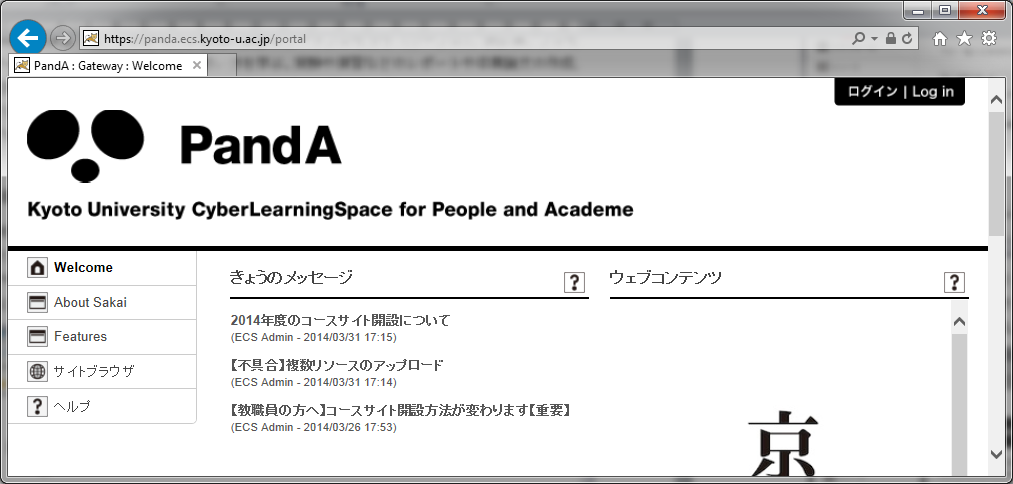
\includegraphics[width=13cm]{TeX_files/figs1/PandA1.png}
\caption{
\label{fig:PandA1}
PandA ログイン画面。右上のログインをクリックし、ECS-IDおよびパスワードを入力してログインする。}
\end{figure}

\begin{figure}
\centering
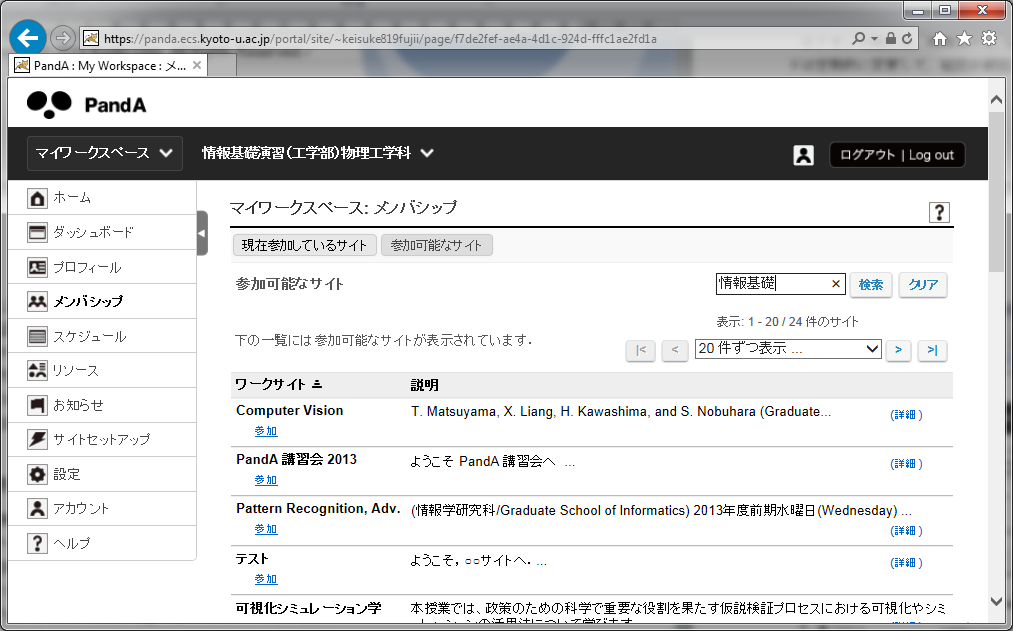
\includegraphics[width=13cm]{TeX_files/figs1/PandA2.png}
\caption{
\label{fig:PandA2}
左の欄の「メンバシップ」をクリックし、次に画面上部の「参加可能なサイト」をクリックしてワークサイトの一覧を表示させる。
一覧から「情報基礎(工学部)物理工学科」を探し(検索も可能)、「参加」をクリックする。}
\end{figure}

\begin{figure}
\centering
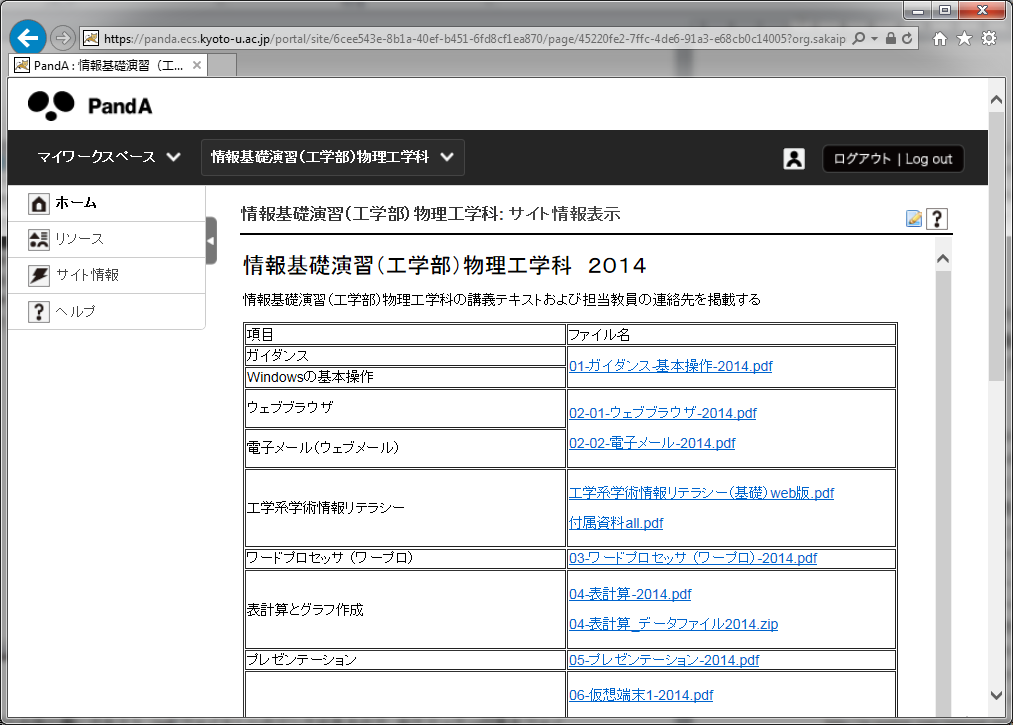
\includegraphics[width=13cm]{TeX_files/figs1/PandA3.png}
\caption{
\label{fig:PandA3}
表の右側の欄にテキスト (pdfファイル) へのリンクがあるので、右クリック→対象をファイルに保存で自分のMドライブ(マイドキュメントフォルダ)に保存しておくとよい。また次回からは、講義HPのURL
https://panda.ecs.kyoto-u.ac.jp/portal/site/6cee543e-8b1a-40ef-b451-6fd8cf1ea870/
をブラウザに入力し、PandAにログインすると、テキスト掲載ページが表示される。
}\end{figure}

 
講義中に分からないことはその時にどんどん質問すること。担当教員以外にもTA(ティーチングアシスタント)と呼ばれる大学院生(あなたたちの先輩)もいる。
 
\section{学術情報メディアセンター利用案内}
メディアセンターのPC端末は授業とは関わりなく全学生が利用可能である。
PC端末が設置してある場所は「学生のための情報環境活用マニュアル」の付録-5.サテライト配置図(最後のページ)に掲載してある。
「情報基礎演習」以外にもメディアセンターのPC端末を利用して行われる授業があり、また、直接授業では利用しなくても、レポートや課題の作成にPC端末のワープロや計算ソフトなどの利用を前提としている講義もある。
OSはWindows 7を搭載しており、ワープロソフトや表計算ソフトだけでなく、数式処理システムソフトや統計解析ソフト、プログラミング支援ソフトなどがインストールされている。
また、それぞれの部屋に設置されているプリンタを使って作成した文書等を印刷することができる。(一人当たり年間200枚の出力制限有り)
 
\section{利用に関しての注意}
PC端末を利用する際の注意に関しては、「学生のための情報環境活用マニュアル」の3.情報システムの安全で適正な利用のお願いおよび4.PC端末サービスの利用方法に記載してあるので、熟読すること。
中でも以下のことに特に気をつけること。
\begin{enumerate}
\item パスワードの適切な管理

\item コンピュータウィルスへの注意

・ 不審なメールを絶対に開かない。

・ 怪しい Web サイトには行かない。

・ 出所のはっきりしないファイルを開かない。

\item  自身のパソコンのセキュリティ対策
 利用者自身が持っているパソコンについても以下のセキュリティ対策をすること。

・ Windows や Office などソフトウェアは常に最新の修正プログラムを適用する。

・ ウィルス対策ソフトを導入し、常に最新のウィルス定義ファイルに更新する。

・ 自宅などでのネットワークへの接続では、ファイアウォールの設定やインターネットセキュリティソフトなどにより安全性の高い接続を確保する。

・ ウィルス対策、およびインターネットセキュリティの両方の機能を備えたソフトウェアが販売、または配布されているので利用するとよい。

シマンテック インターネットセキュリティ(有料)

\url{http://jp.norton.com/internet-security}

トレンドマイクロ ウイルスバスター(有料)

\url{http://safe.trendmicro.jp/purchase/vb.aspx/}

キングソフト インターネットセキュリティ(無料)

\url{http://www.kingsoft.jp/is/index.html}

アバスト! アンチウイルス(無料)

\url{http://www.avast.co.jp/index}
\end{enumerate}

\section{ファイル交換ソフトの使用禁止}
Winny, WinMX, Shareなどのファイル交換ソフトは著作権等の問題となっている。
そのため、PC端末におけるファイル交換ソフトの使用は禁止する。使用できないソフトウェアについては、「学生のための情報環境活用マニュアル」3.4 ネットワーク利用上の注意を参照。
P2Pシステムの使用禁止

Skype などの P2P システムについても、メディアセンターの PC端末では使用を原則禁止します。

その他、疑問点については「学生のための情報環境活用マニュアル」の付録(45ページ~)を参照するか、担当教員に相談する、もしくはメディアセンターに連絡する。


メディアセンター(情報環境機構)の連絡先

075-753-7400

URL:https://www.iimc.kyoto-u.ac.jp/ja/inquiry/
 
 
平成28年度情報基礎演習 担当教員
\begin{table}[htb]
  \begin{tabular}{lll}
  藤井 恵介 &(ふじい けいすけ)	& \url{fujii_at_me.kyoto-u.ac.jp} \\
  安部 豊 & (あべ ゆたか) & \url{yutaka_abe_at_nucleng.kyoto-u.ac.jp} \\
  沖野 真也 & (おきの しんや) & \url{okino.shinya.8n_at_kyoto-u.ac.jp} \\
  池之上 卓己 &(いけのうえ たくみ)&\url{ikenoue.takumi.4m_at_kyoto-u.ac.jp}\\
  市川 和秀&(いちかわ かずひで) &\url{kazuhide_at_me.kyoto-u.ac.jp}\\
  \end{tabular}
\end{table}

\section{補足1. パソコンを買う際のアドバイス}
上にあるように、PC端末にはワープロソフト、表計算ソフトおよびプレゼンテーションソフトがインストールされている。
これら3つのソフトは今後もよく利用するので、家のパソコンにもインストールしておくとよい。
特に、これから新しいパソコンを買う際、ワープロソフト、表計算ソフト(MicrosoftでいうWordとExcel)は一緒についてくるパッケージが多いが、プレゼンテーションソフト(Powerpoint)は最小パッケージにはついていない可能性が高いので、プレゼンテーションソフト付きのパッケージを購入するとよい。
(Microsoft にもOffice Personal with PowerpointやOffice Standardなどのパッケージがある。)
後から、プレゼンテーションソフトのみを買うと価格が高い。

\section{補足2. WindowsとMac}
現在販売されているパソコンは、OSの種類によって大きく2つに分けられる。
WindowsとMacである。パナソニックなどの日本のメーカが販売しているパソコンにはWindows(Microsoft製OS)がインストールされている。
一方、iPhone等で知られるApple Computer から販売されているものが(通称)Macである。
世界のユーザーの9割以上がWindowsユーザーと言われているので、通常はWindowsを購入する方が良い。
一部のマニアックな人々(大学の先生やクリエイターと呼ばれる人たちなど)はMacを使っている。
